Cette zone contient un tableau des morceaux de dump déjà décodés. Cette zone est intimement liée au menu Labels.

Pour ajouter un nouveau champ, il faut sélectionner la zone avec le curseur de la souris dans la vue texte, puis lui définir un nom. L'appui sur le bouton Add ajoute au tableau des labels une entrée avec le nom saisi, la zone définie par la souris et l'encodage courant.
Si une erreur s'est glissée dans vos données, vous pouvez :
\begin{description}
	\item[Editer la ligne] \hfill \\
	il suffit de double cliquer dessus. La fenètre Edit Label (figure \ref{editlabel}) s'affiche alors. Il n'y a plus qu'a renseigner les informations correctes. A noter que le champ "Value" n'est pas éditable et ne sert qu'a vérifier les informations.
	
	\begin{figure}[!h]
		\begin{center}
		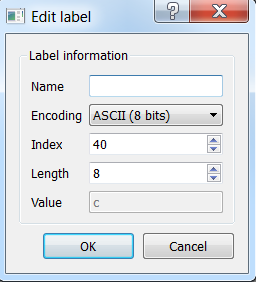
\includegraphics[width=\textwidth]{Edit_label.png}
		\caption{Fenètre d'édition des labels}
		\label{editlabel}
		\end{center}
	\end{figure}
	
	\item[Supprimer la ligne] \hfill \\
	Cette action est disponible en cliquant sur "Labels/Remove Label".

\end{description}
 
 Une fois l'analyse terminée, il convient de sauvegarder les données trouvées. Les fonctions "Labels/Save Mask" et "Labels/Save Mask as ..." permettent d'enregistrer le tableau de labels sous forme d'un masque; c'est à dire uniquement les données indépendantes du Dump, pour qu'il soit réutilisable.
 Les masques ainsi créés peuvent être ouvert et utilisé grâce à la fonction "Labels/Open Mask". Leur format est détaillé dans la documentation technique du projet, dans le cas où vus voudriez créer un masque à partir de spécifications techniques. Il n'est cependant nullement nécessaire de savoir cette information pour utiliser le logiciel.